\section*{Zahnbürstenroboter} 
\hypertarget{bristlebot}{}
\label{bristlebot}
\NewsAuthor{Windell H. Oskay, Ph.D.}


\textbf{\href{http://www.evilmadscientist.com/about/}{\textit{Windell "Evil Mad Chief Scientist" Oskay [1]}} zeigt in diesem Tutorial wie man Roboter aus Zahnbürsten baut, so genannte \textit{Bristlebots}} \\

Der englischsprachige Original Artikel ist copyright-geschützt von \href{http://www.evilmadscientist.com/about/}{\textit{Windell Oskay [1]}} und erschien erstmals am 19.12.2007 auf seiner \href{http://www.evilmadscientist.com/go/bristlebot}{\textit{Homepage [2]}}. Übersetzung von \href{http://spielend-programmieren.at}{\textit{Horst JENS [3]}} mit freundlicher Genehmigung des Autors.

\begin{center}
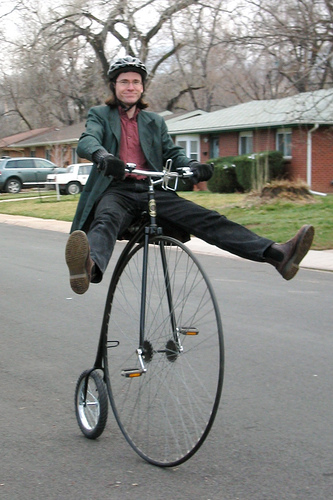
\includegraphics[width=\linewidth]{bristlebot/bristlebot-evilmadscientist.jpg}\\
\footnotesize{Windell Oskay, Ph.D. Bildrechte: [1]}
\end{center}

(Beginn der Übersetzung) \\

Der Zahnbürstenroboter (BristleBot) ist ein einfacher, kleiner, emsiger Roboter. Zutaten: Eine Zahnbürste, eine Batterie, und ein Vibrationsmotor. Das Resultat kann man \href{http://youtu.be/rUSTXUis_ys}{\textit{auf Youtube bewundern [4]}}.

\begin{center}
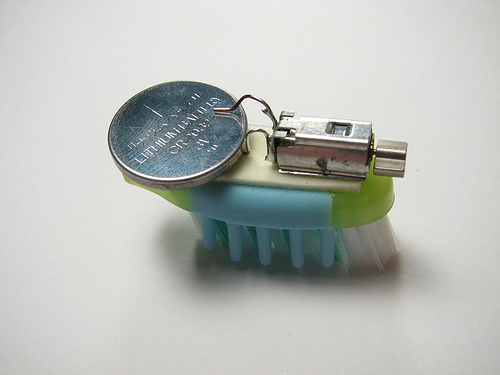
\includegraphics[width=\linewidth]{bristlebot/bristlebot1.jpg}\\
\footnotesize{Bristlebot. Bildrechte: [1]}
\end{center}

Der BristleBot ist unser Versuch einen \href{http://makezine.com/projects/make-10/vibrobots/}{\textit{Vibrobot [5]}} zu bauen: primitive Roboter die durch einen einzigen Vibrations(Exzentrik)-Motor bewegt werden. Sehenswerte Varianten davon sind z.B. der mint-tin (siehe Make Magazin) und der \href{http://www.finkbuilt.com/blog/kids-art-bot/}{\textit{Kid's draw bot [6]}}: ein Vibrobot mit Beinen aus Bleistiften. \\
 
\begin{center}
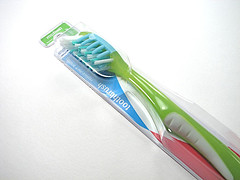
\includegraphics[width=\linewidth]{bristlebot/bristlebot2.jpg}
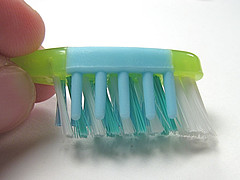
\includegraphics[width=\linewidth]{bristlebot/bristlebot3.jpg}\\
\footnotesize{Zahnbürste mit schrägen Borsten. Bildrechte: [1]}
\end{center}

Zu Anfang steht naturgemäß die Zahnbürste. Wir brauchen eine Zahnbürste deren Borsten alle mehr oder weniger schief geneigt sind (nicht senkrecht). Möglicherweise funktioniert auch ein Bristlebot mit senkrechten Borsten die man von Hand biegt, aber ich habe es nicht versucht. Wenn die Borsten unterschiedlich lang sind ( wie auf den Fotos) brauchen wir vielleicht eine Schere um alle Borsten gleich lang zu stutzen. \\
 
\begin{center}
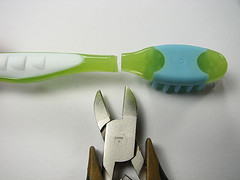
\includegraphics[width=\linewidth]{bristlebot/bristlebot4.jpg}\\
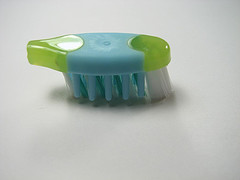
\includegraphics[width=\linewidth]{bristlebot/bristlebot5.jpg}\\
\footnotesize{Bürstenkopf abschneiden. Bildrechte: [1]}
\end{center}

Schneide den Griff der Zahnbürste ab, sodaß nur eine kleine Roboterplattform übrigbleibt. \\ 

Nächster Punkt: Wir brauchen einen Virbrationsmotor oder einen anderen winzigen Moter mit einer Unwucht an der Drehachse. Wenn Du einen genügend kleinen Motor findest kannst du das Gewicht der Unwucht notfalls selbst dran montieren. Man findet solche Motoren z.B. für Pager in allen möglichen Größen. Ich habe meinen für ein paar Dollar auf Ebay bekommen, schau mal dort nach.
\\
\begin{center}
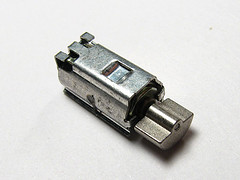
\includegraphics[width=\linewidth]{bristlebot/bristlebot6.jpg}\\
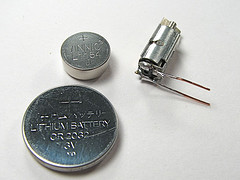
\includegraphics[width=\linewidth]{bristlebot/bristlebot7.jpg}\\
\footnotesize{Vibrationsmotor. Bildrechte: [1]}
\end{center}

Der Motor den ich bekommen habe lief zufrieden mit fast jeder herkömmlichen Spannung von 1 bis 9 Volt. Als Stromquelle funktionieren Alkaline oder Lithium-Batterien (Uhr-Batterien) mit 1,5 Volt oder 3 Volt. Um den Motor an die Batterie anzuschließen habe ich einen Lötkolben benutzt und etwas Kupferdraht an die Motordrähte gelötet.
\\ 

Außerdem brauchen wir Doppelklebeband. Gib einen kleinen Streifen davon auf die Oberseite der Zahnbürste (die Roboterplattform) auf welcher der Motor aufliegt. \\ 

\begin{center}
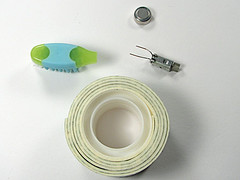
\includegraphics[width=\linewidth]{bristlebot/bristlebot8.jpg}\\
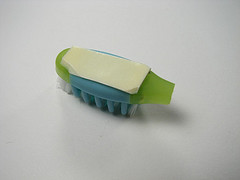
\includegraphics[width=\linewidth]{bristlebot/bristlebot9.jpg}\\
\footnotesize{Doppelklebeband. Bildrechte: [1]}
\end{center}

Klebe den Motor auf das Klebeband. Das Klebeband sorgt für Abstand damit das Unwucht-Gewicht nicht auf die Zahnbürste hämmert. Außerdem sorgt das Klebeband für eine starke, flexible Verbindung welche die starken Vibrationen des Roboters aushält. Eine erste Verbindung zur Batterie ist möglich indem man die Batterie einfach draufstellt - das ist allerdings nicht sehr stabil und sie wird bald runterfallen.
\\ 

Eine bessere Methode ist es einen der Drähte runterzubiegen zum Klebeband, sodaß man die Batterie draufkleben kann und trotzdem eine elektrisch leitende Verbindung schafft. Mit dem anderen Draht die andere Seite der Batterie berühren und es kann los gehen. \\

\begin{center}
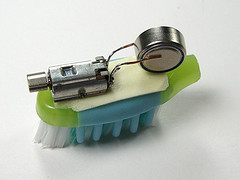
\includegraphics[width=\linewidth]{bristlebot/bristlebot11.jpg}\\
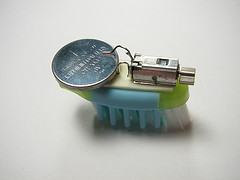
\includegraphics[width=\linewidth]{bristlebot/bristlebot13.jpg}\\
\footnotesize{Batterien. Bildrechte: [1]}
\end{center}
Der vollendete BristleBot, aktionsbereit. Wenn Du einen Bristlebot laufen lässt merkst Du dass er eine Tendenz hat nach rechts oder links zu steueren. Das wird beeinflusst durch Borstenlänge (z.B. eine einzelne lange Borste), die Position von Motor und Batterie und auf welcher Seite man die Batterie anschliesst. Drehe die Batterie einmal um wenn der Bristlebot nicht vernünftig läuft.
\\  

Nur zur Erinnerung: Dies ist einer von vielen verschiedenen Arten von Vibrobots - da draußen gibt es viele andere Varianten wenn du nur suchst. Wir haben viele andere Varianten gesehen oder davon gehört, und wir wissen dass Bürsten mit schiefen Borsten schon zuvor als Antrieb verwendet wurden. Diese spezielle Variante ist vielleicht einzigartig, auf jeden Fall spaßig. Nur wenige Roboter die man selbst so einfach bauen kann sind so belohnend. Mit den richtigen Teilen kannst du einen in ein paar Minuten bauen. Mach eine Horde davon und lass sie um die Wette rennen !
\
\begin{center}
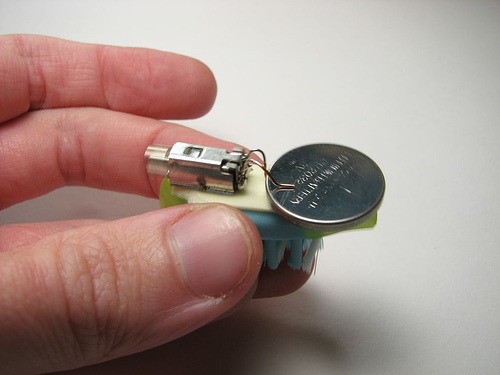
\includegraphics[width=\linewidth]{bristlebot/bristlebot14.jpg}
\footnotesize{Bristle Bot. Bildrechte: [1]}
\end{center}

(Ende der Übersetzung) \\

\subsection*{Fachbegriffe:}

~~~\textbf{Vibrobot} von Vibrations-Roboter. \\

\textbf{Bristlebot} von engl. bristle = Bürste. \\


\subsection*{Download, Feedback:}
\textbf{R.I.S.-Journal}, Ausgabe 001: \\
\href{http://spielend-programmieren.at/de:ris:001}{spielend-programmieren.at/de:ris:001}\\
\textbf{Download} Ordner, verschiedene Formate: \href{http://spielend-programmieren.at/risjournal/001/bristlebot}{\texttt{spielend-programmieren.at/\\risjournal/001/bristlebot}} \\
\textbf{Feedback} \Letter\ \texttt{drwho@evilmadscientist.com}\\
                                   

\subsection*{Lizenz der Übersetzung, Quellen}
\begin{wrapfigure}{l}{2.0cm}

\includegraphics[width=2cm]{ccbysa88x31.png}
\end{wrapfigure}
Dieses Material steht unter der Creative-Commons-Lizenz Namensnennung - Weitergabe unter gleichen Bedingungen 4.0 International. Um eine Kopie dieser Lizenz zu sehen, besuchen Sie \url{http://creativecommons.org/licenses/by-sa/4.0/deed.de}. \\

\textbf{Quellen:}\\
{[}1{]} \href{http://www.evilmadscientist.com/about/}{evilmadscientist.com} \\
{[}2{]} \href{http://www.evilmadscientist.com/go/bristlebot}{evilmadscientist.com/go/bristlebot} \\
{[}3{]} \href{http://spielend-programmieren.at}{spielend-programmieren.at} \\
{[}4{]} \href{http://youtu.be/rUSTXUis_ys}{youtu.be/rUSTXUis\_ys} \\
{[}5{]} \href{http://makezine.com/projects/make-10/vibrobots/}{makezine.com/projects/make-10/vibrobots} \\
{[}6{]} \href{http://www.finkbuilt.com/blog/kids-art-bot/}{finkbuilt.com/blog/kids-art-bot} 

